\documentclass[11pt]{article}
\usepackage{latexsym}
\usepackage{amsmath}
\usepackage{amssymb}
\usepackage{amsthm}
\usepackage{epsfig}
\usepackage[tight]{subfigure}

\usepackage{amsmath}

\DeclareMathOperator*{\minimize}{min}
\DeclareMathOperator*{\maximize}{max}

\usepackage{algorithm}
 %on linux you may need to run sudo apt-get install texlive-full to install algorithm.sys
\usepackage{algorithmic}

\usepackage{verbatim}

\newcommand{\handout}[5]{
  \noindent
  \begin{center}
  \framebox{
    \vbox{
      \hbox to 5.78in { {#1} \hfill #2 }
      \vspace{4mm}
      \hbox to 5.78in { {\Large \hfill #5  \hfill} }
      \vspace{2mm}
      \hbox to 5.78in { {\em #3 \hfill #4} }
    }
  }
  \end{center}
  \vspace*{4mm}
}

\newcommand{\lecture}[5]{\handout{#1}{#2}{#3}{#4}{#5}}
\newcommand{\collision}[0]{\mathrm{collision}}
\newcommand{\nocollision}[0]{\overline{\collision}}

\newcommand*{\QED}{\hfill\ensuremath{\square}}

\newtheorem{theorem}{Theorem}
\newtheorem{corollary}[theorem]{Corollary}
\newtheorem{lemma}[theorem]{Lemma}
\newtheorem{observation}[theorem]{Observation}
\newtheorem{proposition}[theorem]{Proposition}
\newtheorem{definition}[theorem]{Definition}
\newtheorem{claim}[theorem]{Claim}
\newtheorem{fact}[theorem]{Fact}
\newtheorem{assumption}[theorem]{Assumption}
\newtheorem{note}[theorem]{Note}

% 1-inch margins, from fullpage.sty by H.Partl, Version 2, Dec. 15, 1988.
\topmargin 0pt
\advance \topmargin by -\headheight
\advance \topmargin by -\headsep
\textheight 8.9in
\oddsidemargin 0pt
\evensidemargin \oddsidemargin
\marginparwidth 0.5in
\textwidth 6.5in

\parindent 0in
\parskip 1.5ex
%\renewcommand{\baselinestretch}{1.25}

\begin{document}

\lecture{Statistical Techniques in Robotics (16-831, S22)}{Lecture \#22
  (Monday, April 11)}{Lecturer: Kris Kitani}{Scribes: Mansi Agarwal, Ashwin Misra}{Imitation Learning}

\section{Review}
In review, the last few lectures were on Reinforcement Learning. Reinforcement Learning is a learning paradigm where an agent tries to learn an optimal, or nearly-optimal, policy that maximizes short-term and long term rewards.  Theoretically, we often assume the RL environment as a Markov Decision Process(MDP).

The three main types of Reinforcement Learning Algorithms, namely-
\begin{itemize}
    \item Policy-based Methods- In these methods, the stochastic policy is directly learned from the state and actions. The actions are taken by sampling from the policy.We explicitly build a representation of a policy (mapping $\pi: s \rightarrow a)$ which maps the state to action, and keep this in cache while the learning is happening.
    \item Hybrid-based methods- In these methods, the policy proposes a set of possible actions that can be taken for a given state and the feasibility is calculated by the estimated value function, which evaluates the actions taken based on the given policy.
    \item Value-based methods- These methods don't learn the policy but learn the states or state-action values. The action is chosen by the best reward in that state. Due to this, it is necessary that all the actions are explored for the state.Unlike the policy based methods, the policy is not stored in the cache, only the value function. This value function is used to derive the policy.
\end{itemize}

Depending on the underlying assumptions of the problem that we have, RL algorithms can also be classified into- 
\begin{itemize}
    \item Model-based RL Algorithms: Such algorithms have full access to the environment including state transition dynamics and reward function.  Such algorithms represent the environment as a Markov Decision Process. Value based or policy based iteration algorithms come under model-based algorithms. In policy iteration, the rewards (used to estimate the policy or value functions) are not the result of the interaction with the environment but directly given by the reward function (accessible to the algorithms). Furthermore, since we have access to the dynamics model, the agent need not interact with the environment to retrieve the next state given current state-action pair.
    
    \item Model-free RL Algorithms: Such algorithms do not have access to the dynamics model (state transition dynamics) and can only draw samples from the environment. Model-free methods, such as Monte Carlo methods do not use have access to dynamics model, even though the assumption that the environment can be represented as an MDP is implicitly made. There can be two kinds of model-free algorithms: off-policy vs on-policy. On policy algorithms are those algorithms where the policy needs to be updated after every parameter update and the updated policy needs to interact with the environment for updated sample trajectories., i.e., every time the policy parameters are updates, the agent has to collect more data and cannot use the past experience. On the other hand, off policy algorithms are those where no new data needs to be collected after a policy parameter update. In such algorithms, there are often two policies, one that interacts with the environment to sample trajectories and the other that is optimised using the experience of the other policy. There is an assumption of full coverage between the two policies. 
    
\subsection{Last Lecture}
In the last lecture, we went through Policy gradient methods- namely Monte Carlo Policy Gradient and REINFORCE. Policy Gradient methods don't require models and learn from interactions. They take the estimated return in the gradient to update the policy step. We see how large rewards result in large gradient variance, and how it can be solved with enforcing causality or a baseline offset. And when the value function estimates are used as the baseline, for policy gradient methods, the methods are called actor-critic methods. These methods use a function approximator return estimate in their policy update step. As discussed before in the hybrid policy based methods, the critic is the evaluation of the actions to take which is done by the value function, and the actor is the policy which gives us possible actions to take from a state.







\end{itemize}
%This section serves as a review of the previous lecture and any other context required to frame the content of the current lecture. 

%You may format the scribes in any way you like, aside from changing font style, size and page format. Please use subsections and paragraphs to increase the readability of your notes.

%Length requirement 1-2 pages.
        

\section{Summary}
\subsection{Imitation Learning}
\subsubsection{Why Imitation Learning?}


Reinforcement learning is a widely used machine learning paradigm where an agent learns from its own experience. The agent perceives the state, and using a policy it takes the next action. Based on this action, it receives a reward and the environment transitions to the next state. Reinforcement learning algorithms aim at learning the optimal policy which maximises long term as well as short term rewards. Typically, RL methods work well when the state and action space is small and finite. However in most cases, it is tough to deploy RL algorithms. For example, in situations where reward is only obtained after the last step in the horizon (say a game of chess where the reward is 0 or 1 depending on whether the agent lost or won). There could also be scenarios where constructing a reward function is complex and not intuitive. Furthermore, even if we have access to a reward function that returns rewards at every step, RL algorithms can take a long time to converge since they start from trial and error and try to figure out what's best in a given scenario through experience (interacting with the environment).

A feasible solution to all these problems is Imitation Learning (IL). Imitation Learning is also known as Learning from Demonstration, Apprenticeship Learning, Behavior Cloning, and Inverse Reinforcement Learning. In Imitation Learning, the agent learns a policy from demonstrated expert behavior. So, the goal of IL is same of RL to learn an optimal policy but instead of using its own experience, it learns from an expert's demonstrations.

As we'll see later, Imitation Learning employs expert demonstrations and henceforth speeds up the learning process (as compared to RL algorithms when the state and action space is not finite). Also, since IL uses demonstrations, there is no need to construct reward functions which saves a lot of time and complexity.

\subsubsection{Problem Formulation}
\normalfont

Let us first formalise the Imitation Learning(IL) problem.
$$
\mathcal{A}_{\mathrm{IL}}:\left\langle\mathcal{D}^{*}, \pi^{*}, \mathcal{T}, \mathcal{R}\right\rangle \rightarrow \pi
$$

Here, $\mathcal{A}_{\mathrm{IL}}$ denotes the Imitation Learning algorithm.
Let us now discuss what each element describes. 

\begin{enumerate}
    \item Expert demonstrations ($\mathcal{D}^{*}$): 
    $$
\mathcal{D}^{*}=\left\{\boldsymbol{\zeta}_{n}\right\}_{n=1}^{N} \sim \mathcal{E} \mid \pi^{*}
$$
    Expert demonstrations are defined as a sequence of variables such as a sequence of states and actions. These sequences are sampled from the optimal policy $\pi^{*}$. The representation form of demonstrations is flexible though, as it could be represented either as 
    $$\text{state sequence}\quad \boldsymbol{\zeta}=\left\{s^{(0)}, s^{(1)}, \ldots, s^{(T)}\right\}$$  
    or 
    $$\text{a sequence of state-action pairs}\boldsymbol{\zeta}=\left\{s^{(0)}, a^{(0)}, s^{(1)}, \ldots, a^{(T-1)}, s^{(T)}\right\}$$
    
    Note that in off-policy RL algorithms, the policy used to sample trajectories might not be optimal, whereas for IL, the optimal policy is employed. Also, these demonstrations do not include rewards. We assume that the action taken per state optimises some underlying function. In other words, the action is the best action possible for the given state. Another thing to pay attention is that these demonstrations might be from one single episode or $N$ episodes, and could also be shuffled. So, it is not necessary that an action $a_1$ on state $s_1$ would lead to state $s_2$ from the sequence.
     
    \item Oracle (Optimal Policy $ \pi^{*}$): 
    $$
    \pi^{*}(a \mid s)
    $$
    Optimal policy is the expert policy where the expert demonstrations are sampled from. One thing to question is that if we have access to the optimal policy, why do we need an algorithm to find the  policy at all? It should be noted that we do not necessarily have access to the optimal policy, but we can get samples from it during training. In other words, we might not have access to the full parameterization of the optimal policy and thereby can only use it to get access to the best action at a given state. Such type of IL is known as Interactive IL. 
  
    
    \item Dynamics function $\mathcal{T}$ and Reward function $\mathcal{R}$: 
    $$
    \mathcal{T}\left(s^{\prime} \mid s, a\right), R\left(s, a\right)
    $$
    The dynamics model and the reward function together constitute the environment $\mathcal{E}$, which still needs to be a Markov Decision Process (MDP). This means that the states in the environment follow the Markov property, where the next state is only dependent on the current state and action and is independent of the previous state and actions. 
     $\mathcal{T}(s’|s,a)$ denotes the transition model which defines the probability that an action $a$ in the state $s$ leads to state $s’$.  Reward function ($R(s,a)$) returns the reward for the state-action pair.
\end{enumerate}

\subsubsection{A Classification on IL Algorithms}

We can roughly divide IL algorithms into three categories depending on which elements (discussed above) the agent has access to.

\begin{table}[h]
\centering
\begin{tabular}{|c|c|c|c|}
\hline
Access to       & Passive IL & Active IL & Interactive IL \\ \hline
Demonstrations $D^*$     & yes        & yes       & optional       \\ \hline
Environment $\varepsilon$ & no         & yes       & yes            \\ \hline
Oracle $\pi^*$           & no         & no        & yes            \\ \hline
Dynamics $T$             & no         & optional  & optional       \\ \hline
Reward $R$               & no         & optional  & optional       \\ \hline
\end{tabular}
\caption{ A Classification on IL Algorithms}
\label{tab:IL-type}
\end{table}


\begin{enumerate}
    \item Passive IL: As we can see from Table \ref{tab:IL-type}, Passive IL only has access to demonstrations. Since, we use the expert demonstrations and supervise our model to clone the behaviour of the expert, passive IL is also known as behavior cloning or supervised learning. So, essentially, we have a set of demonstrations (dataset), we use that to train an ML algorithm and learn the policy. This idea has been employed by researchers since 1960s. It was first discussed in the paper "Pattern Recognising Control Systems" \cite{widrow1964pattern}. Another important example of behaviour cloning is ALVINN (Autonomous Land Vehicle In a Neural Network) \cite{pomerleau1988alvinn}, a vehicle equipped with sensors, which learned to map the sensor inputs into steering angles and drive autonomously. This project was carried out in 1989 by Dean Pomerleau, and it was also the first application of imitation learning in general. More recently, a paper called "Learning by Cheating" \cite{chen2020learning} employed the idea of behaviour cloning to improve autonomous driving. The paper proposes an algorithm that entails two steps. In the first step, the method first trains a "privileged agent" which has access to the full state of the environment including meta-data. Therefore, this step does not need to take care of the perception component of autonomous driving. Once the privileged agent is trained, it is treated as the optimal policy and is then used to sample expert demonstrations. In step 2, the sensorimotor agent is trained using these expert demonstrations via Behaviour Cloning. This method beat the state-of-the-art results. 
    
    The way behavioural cloning works is quite simple. Given the expert’s demonstrations, we divide these into state-action pairs and treat these pairs as independent and identically distributed (i.i.d.) examples. Using supervised learning, we learn the optimal policy. Passive IL lies with online linear classification algorithms with sampled one-shot feedback.
    \begin{figure}[H]
\centering
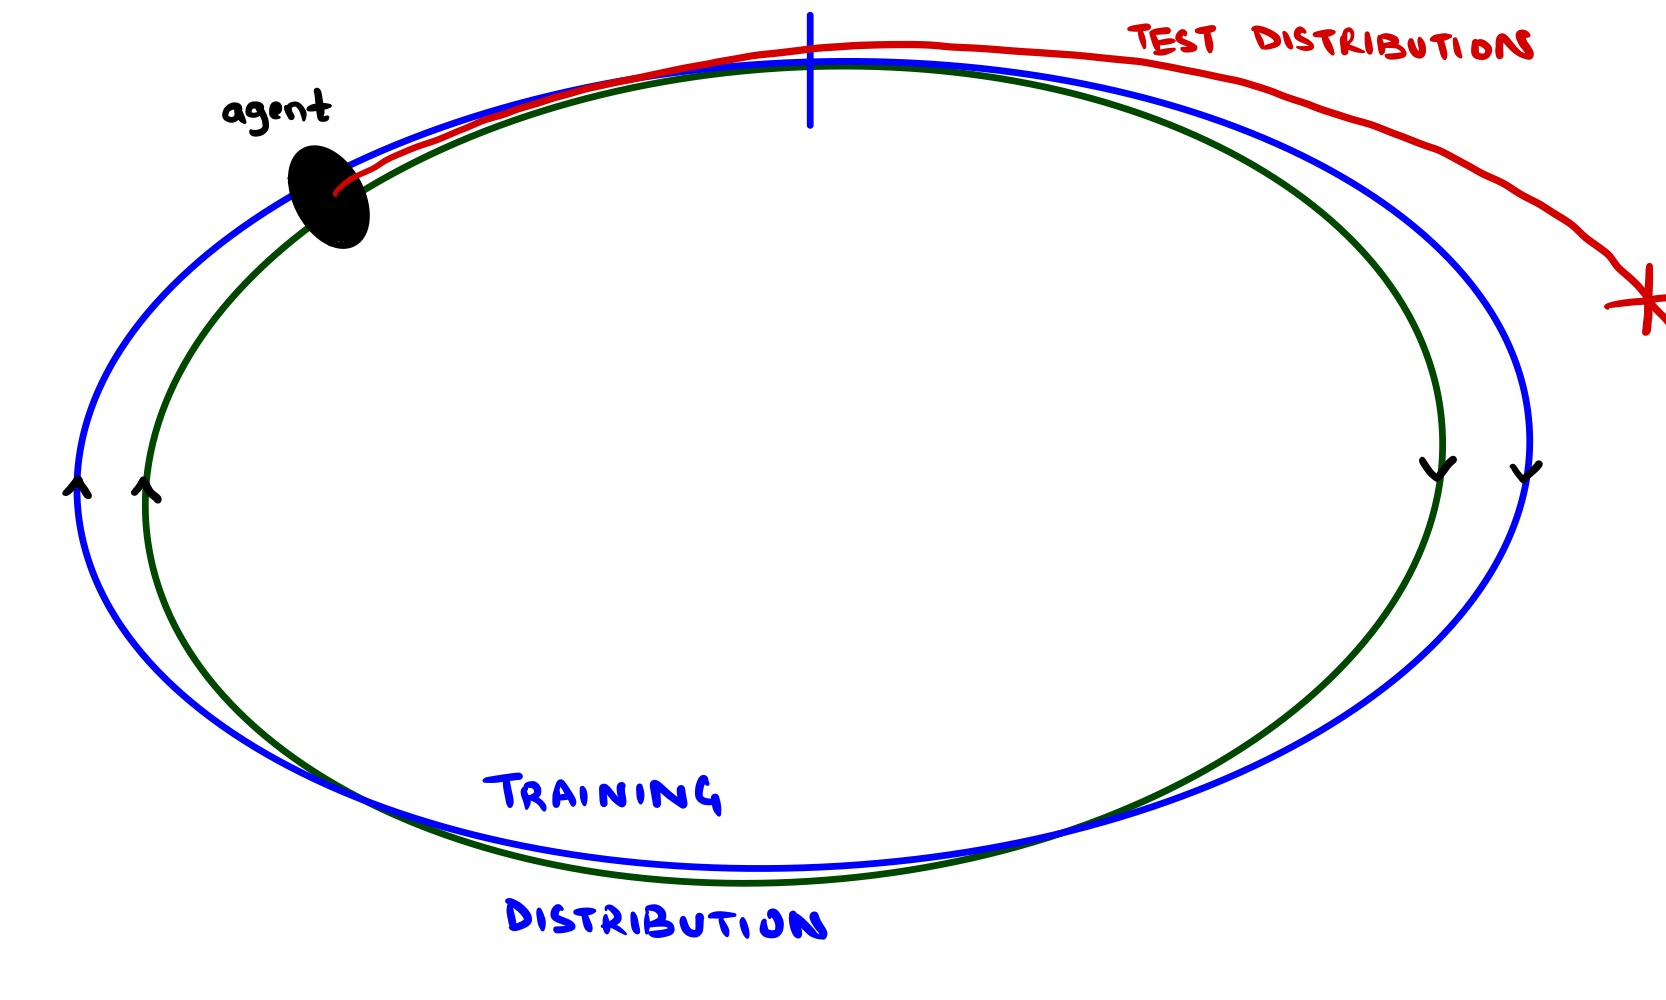
\includegraphics[width=0.8\linewidth]{figs/Image-1(1).jpg}
\caption{Covariate Shift}
\label{fig:ncs}
\end{figure}
    
    Passive IL is simple and intuitive to use but it has a major disadvantage. The learned policy only works well on states it has been trained on. So if one uses a policy trained using Behaviour Cloning for long horizon planning, the method might fail due to this covariate shift. For example, in Fig \ref{fig:ncs}, we see that at every step the policy makes small errors which when accumulated over time result in a shift in test distribution (from the training data distribution). As the errors accumulate, the policy reaches a state it has never seen before. This results in a bogus action which further results in a state the policy has not been trained on thereby, leading to failure. 
    
    Hence, passive IL only models short-term (one-shot) behaviour and cannot model long-term behavior well. We could also say that passive IL works best when 1. The problem is simple 2. The state space is finite and demonstrations cover all possible states. 
    
    \item Active IL:
    Active IL has access to expert demonstrations as well as the environment, but does not have access to the optimal policy. In active IL, the method employs the expert demonstrations to initialise its policy parameters and then interacts with the environment (just like RL algorithms) to further finetune the policy. Paper "Reinforcement Learning of motor skills with policy gradients" \cite{peters2008reinforcement} employs this idea. It first uses behaviour cloning to supervise the agent to learn how to hit a ball using a bat, and then uses RL to improve the agent's performance. This helps in speeding up the process of finding the optimal policy.
    
    \item Interactive IL:
    Interactive IL has all other access to the environment, making the expert demonstrations optional to the agent as it has access to the oracle policy, serving as an alternative of expert demonstrations. In essence, the agent interacts with the environment and there is an interactive oracle feedback to help improve the policy. 
     
\end{enumerate}



\subsection{Inverse Reinforcement Learning}
\subsubsection{Why Inverse Reinforcement Learning}
Inverse reinforcement learning is the process of studying an agent's objectives, values, or rewards with the aid of using insights of its behavior. This algorithm estimates the policy and the reward function by learning from Expert Demonstrations and how they act in the environment. It helps in obtaining a reward function which can be used to generalize to other unknown environments for which reward functions cant be defined easily. This knowledge can be transferred to new but similar environments. For example, a reward function for a self-driving scenario on a busy road cannot be transferred to a robotic manipulation problem.

\begin{figure}[H]
\centering
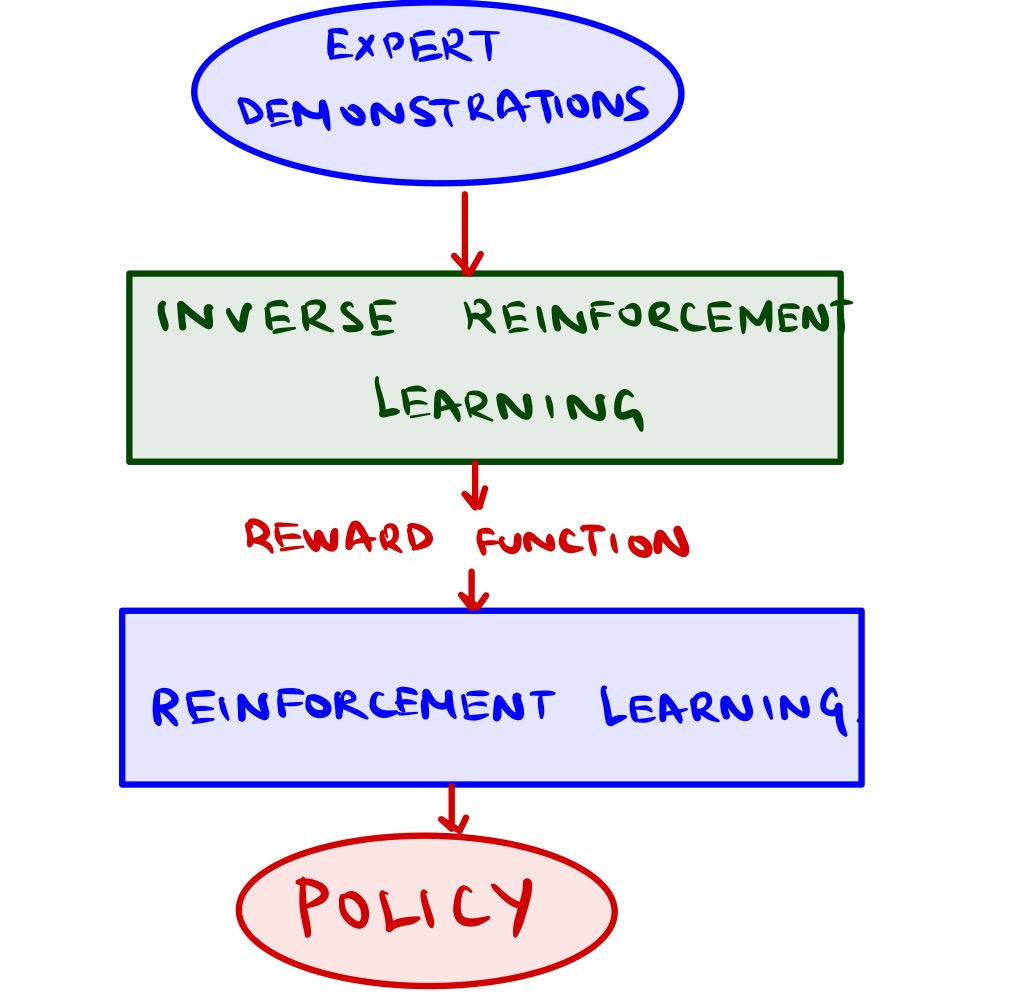
\includegraphics[width=0.8\linewidth]{figs/Image-1.jpg}
\caption{Inverse Reinforcement Learning}
\label{fig:nas}
\end{figure}


\subsubsection{Trajectory Forecasting}
Let us assume a scene in which a squirrel has to reach a nut in a park. The park has a lot of obstacles in it as shown in the figure. We know the start and the end positions and we need to find a path for the squirrel to reach the destination. \newline
\begin{figure}[H]
\centering
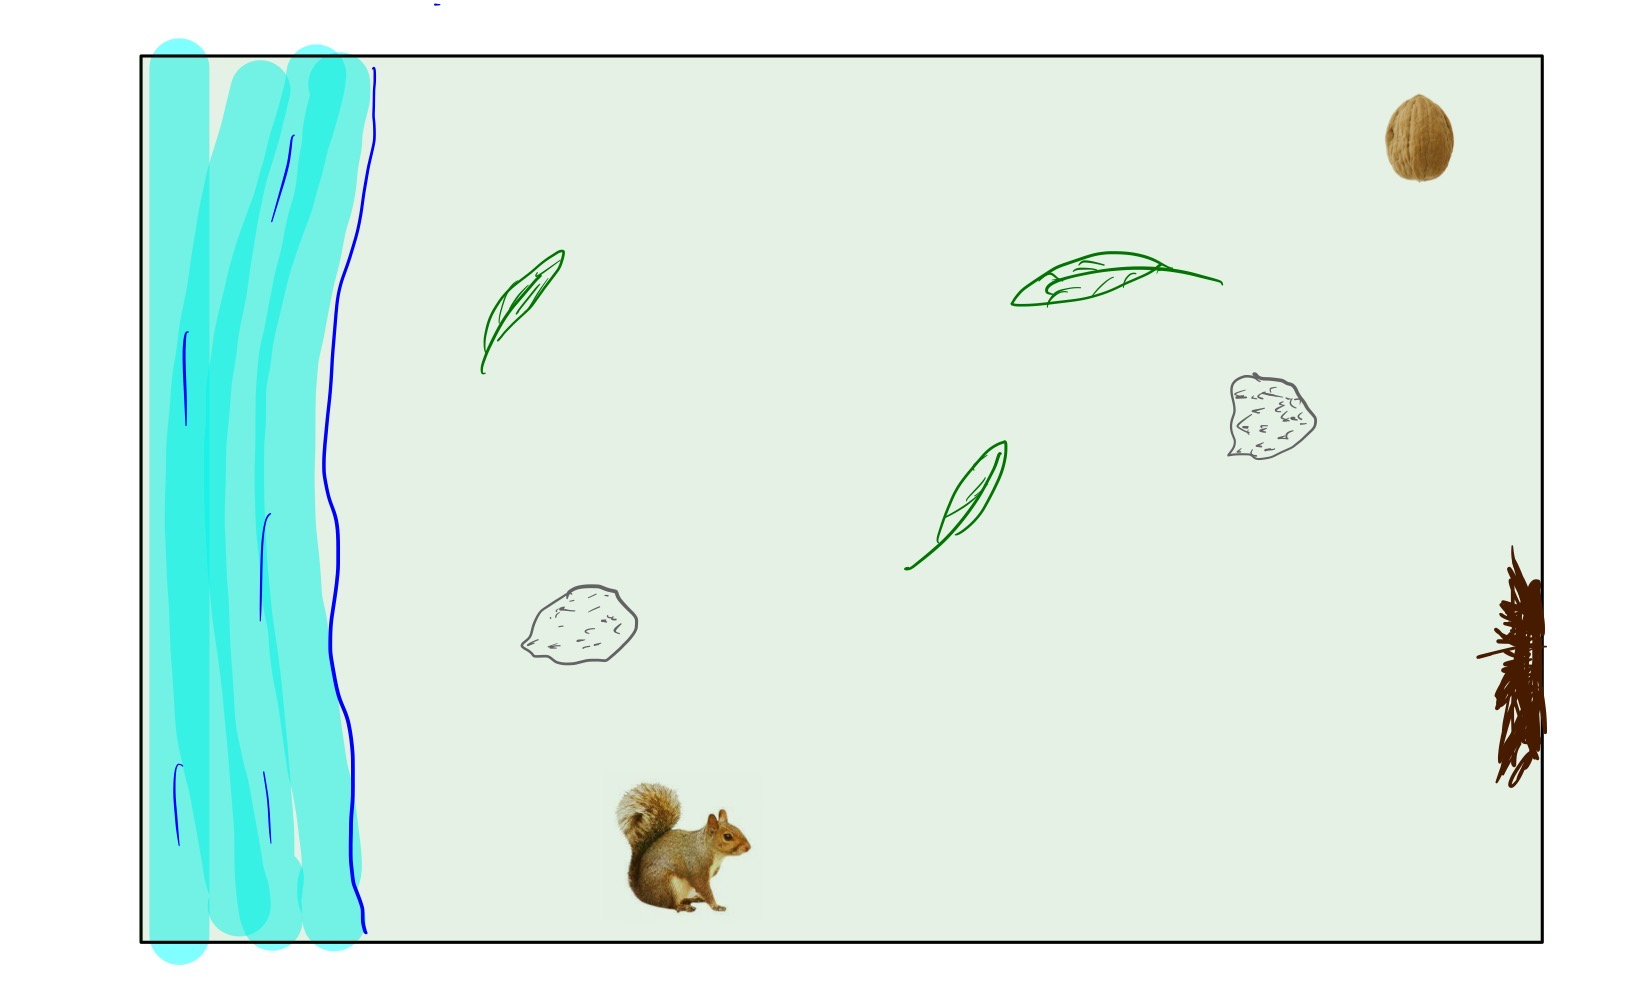
\includegraphics[width=0.8\linewidth]{figs/IMG_0208.JPG}
\caption{Novel scene}
\label{fig:ns}
\end{figure}

The training data that we have is the expert's demonstration and the physical features of the park such as the grass, the stones and the neighboring trees. This input gives the trajectory as the reward function for the squirrel to reach the nut. This same reward function, which is not scene specific, can be used to forecast activities in novel scenes. \newline 

\begin{figure}[H]
\centering
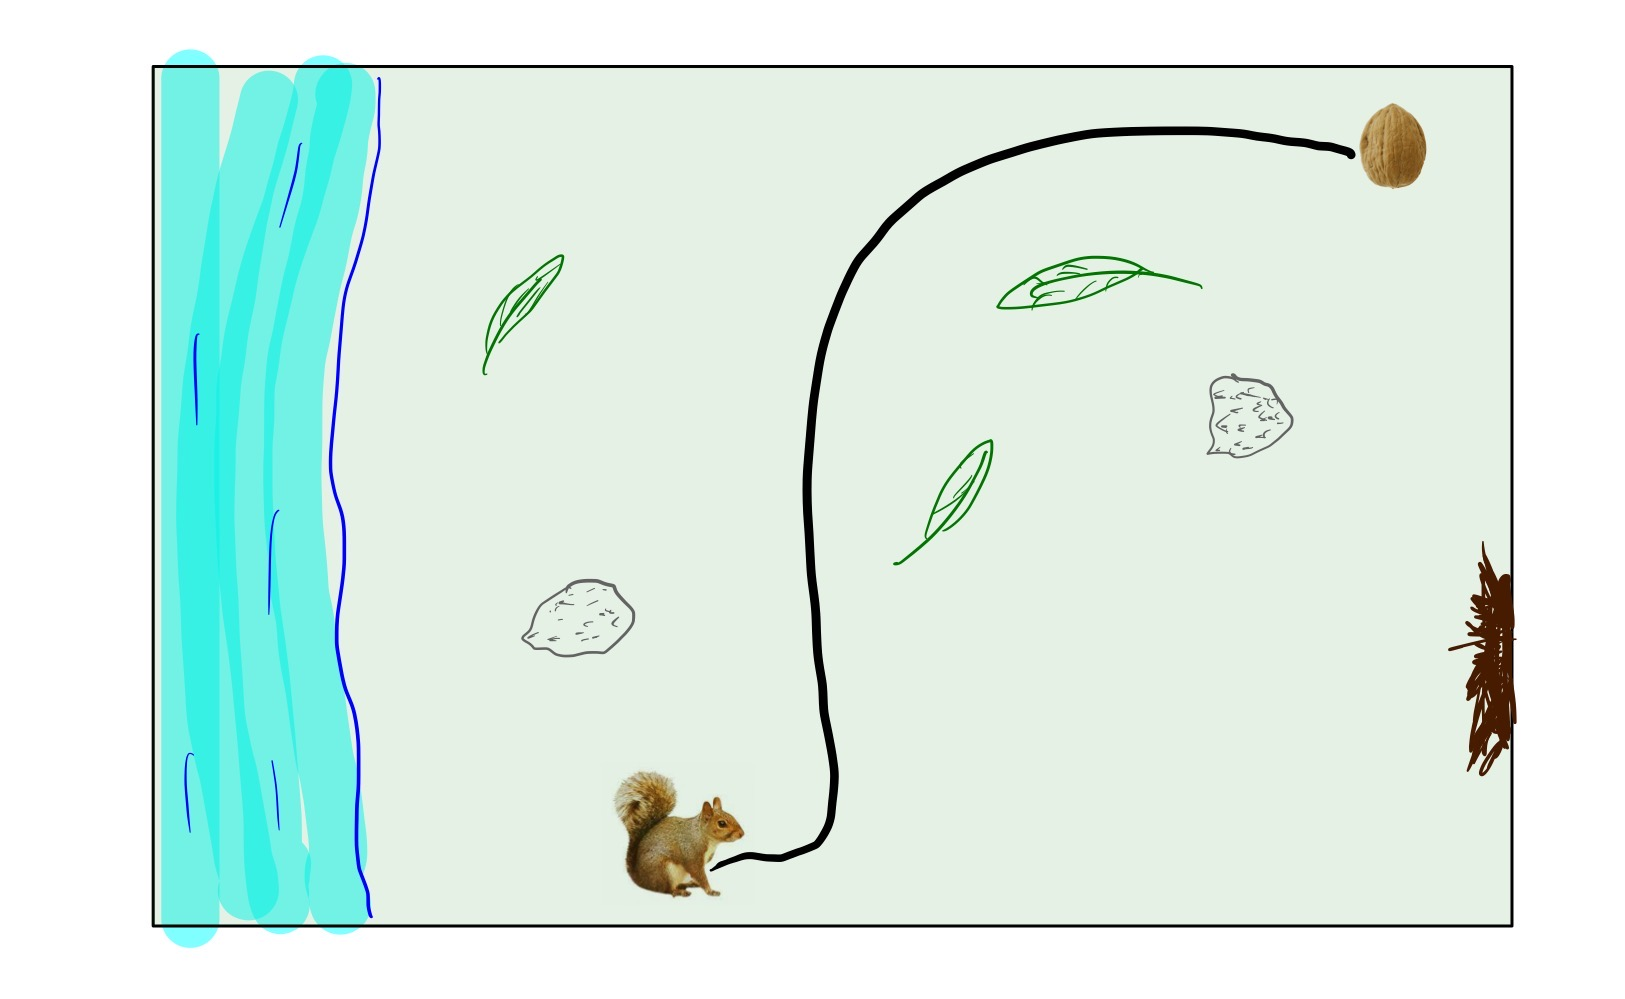
\includegraphics[width=0.8\linewidth]{figs/IMG_0209.JPG}
\caption{Demonstrated Activity}
\label{fig:nsa}
\end{figure}
In this example, This combined with the physical features i.e. the scene segmentation data comprise of the training data.

\begin{figure}[H]
\centering
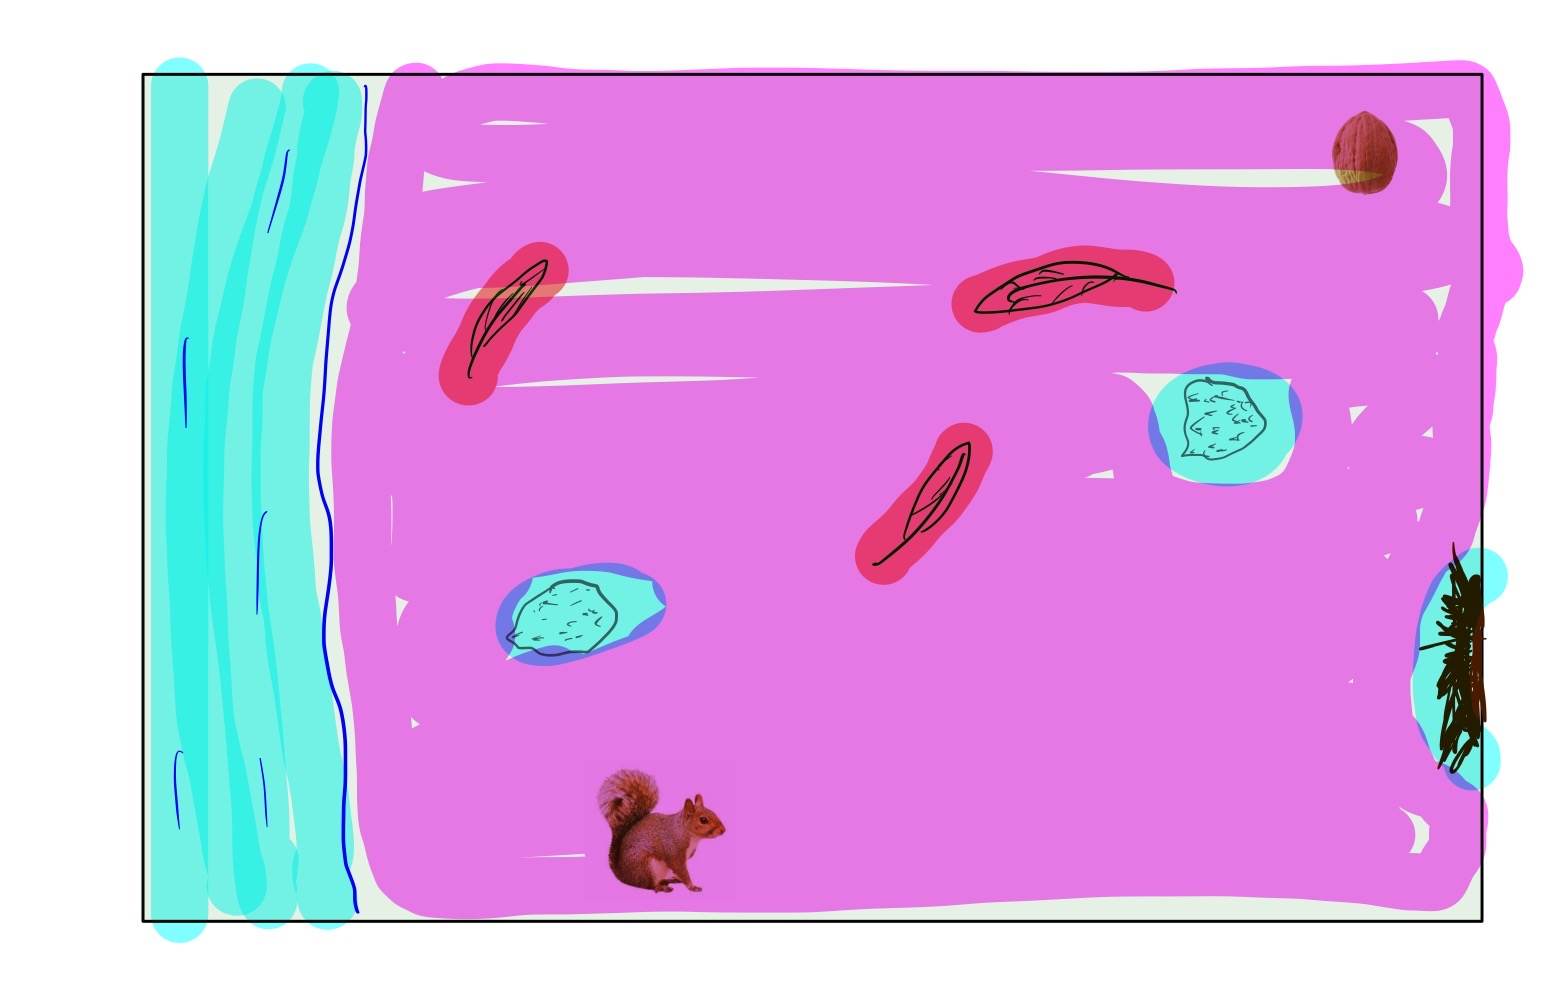
\includegraphics[width=0.8\linewidth]{figs/IMG_0210.JPG}
\caption{Physical Features}
\label{fig:pf}
\end{figure}
Inverse Reinforcement Learning assumes a Markov Decision Process defined over a grid world, which is fitted across the scene. The gridworld on our running example is shown in the figure-
\begin{figure}[H]
\centering
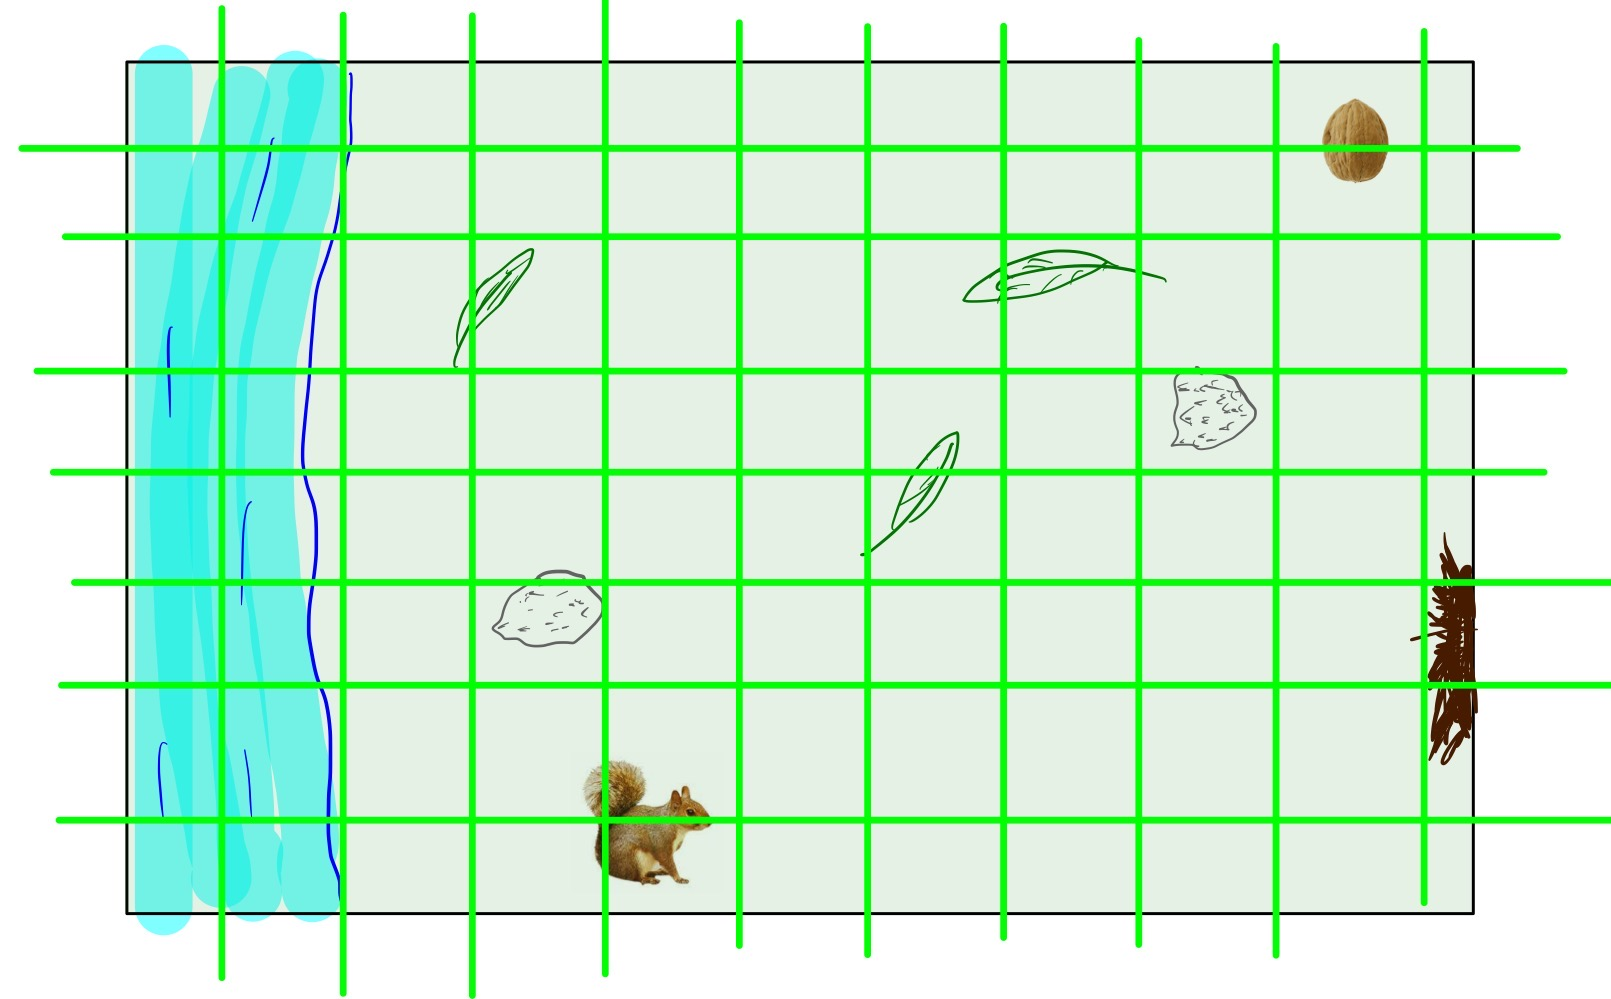
\includegraphics[width=0.8\linewidth]{figs/IMG_0211.JPG}
\caption{MDP defined over a gridworld}
\label{fig:mdp}
\end{figure}
\begin{align*}
    \mathcal{S} = \{x_0, a_0, R(x_0), x_1, a_1, R(x_1),....., x_g, a_g, R(x_g)\}
\end{align*}
where $x=state$, $a=action$, and $R=reward$. The state is the the co-ordinates on the grid, the actions being the velocity in pre-defined directions. The dynamics are the probability of going to state x' from x while we take the action a $P(x' | x,a)$. To further understand the MDP, the features of a state (f(x)) could be the semantic segments of the scene for each location. The value function of each state (V(x)) could be the expected feature reward over a trajectory originating from that state, also known as cost-to-go. \newline
As shown in the figure, the reward function highlights the segments that are high reward and the segments which are low reward. This is the output of the INverse Reinforcement Learning Algorithm.

\begin{figure}[H]
\centering
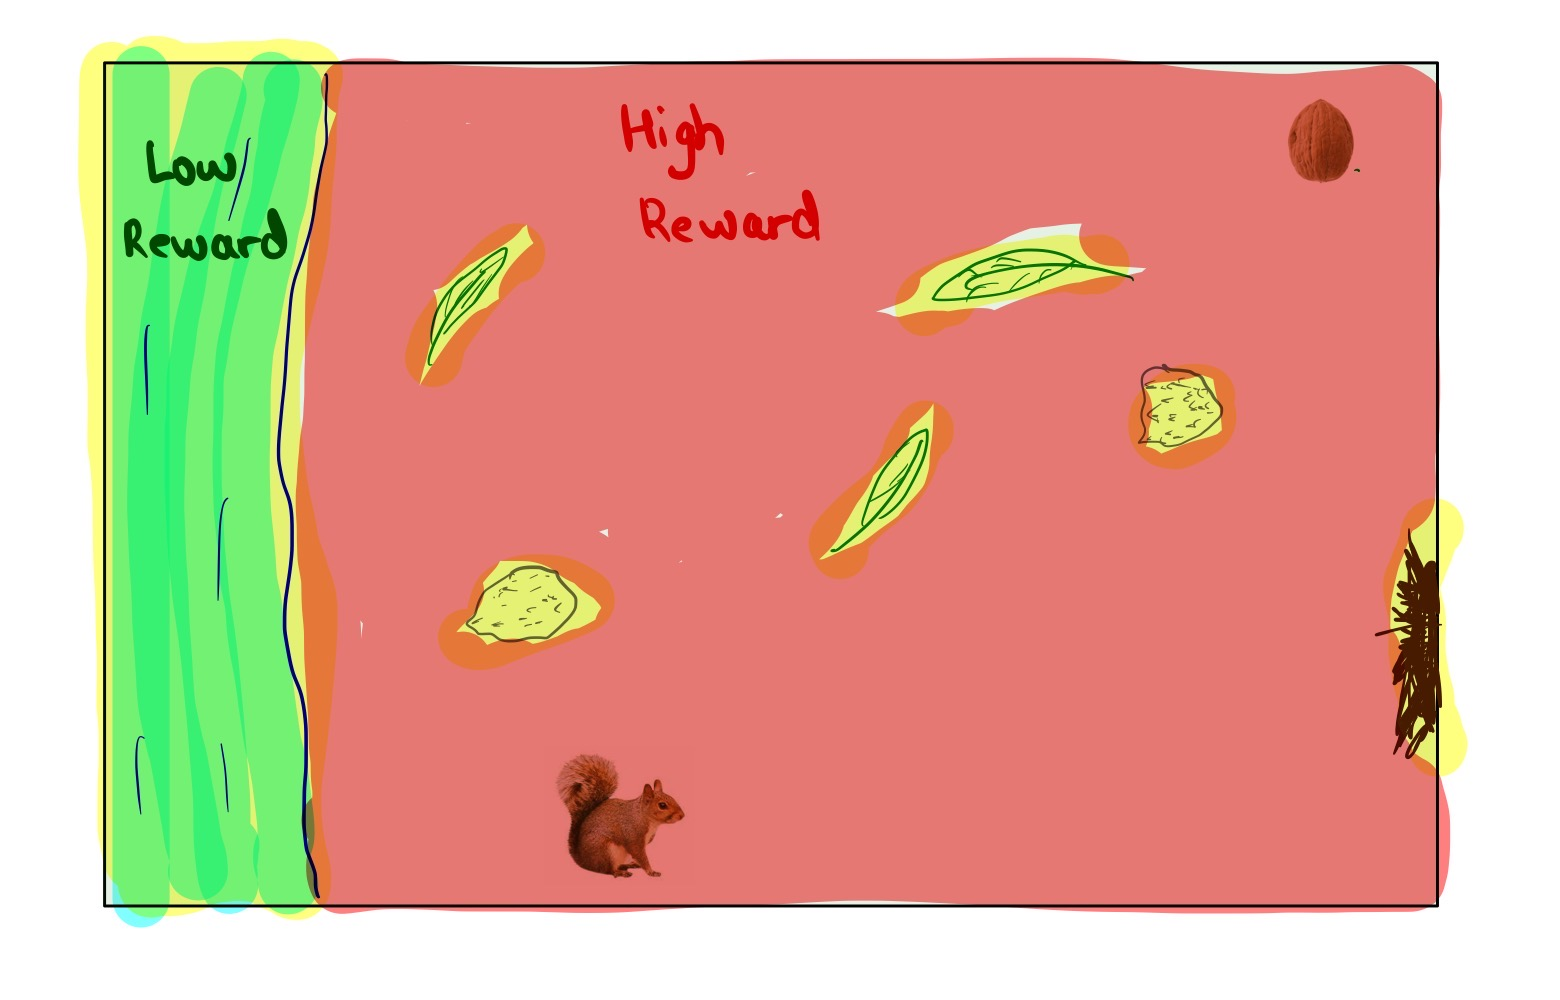
\includegraphics[width=0.8\linewidth]{figs/IMG_0212.JPG}
\caption{Output of IRL}
\label{fig:output}
\end{figure}

%\section*{References}
%Include your references here. Please cite any resources you found useful.	
%Populate the refs.bib file or list your references manually. Be consistent in formatting!
{
\bibliography{refs}
\bibliographystyle{abbrv}
}

\section{Appendix}
%This section provides any relevant background material that was not covered in the lectures, but was found to be useful for understanding the material. 
%For example, derivations, theory underlying techniques employed, etc.

We briefly discussed the problem of covariate shift in Passive IL. Here, we will discuss ways of curbing this problem. 

One way of reducing the covaiate shift is by making the test distribution equivalent to the training distribution. We know that the test distribution comes from the learned policy and the training distribution comes from the expert (optimal policy). Mathematically, we want to make
\begin{align*}
    p_{\pi^{*}}(s_t) = p_{\pi_\theta}(s_t)
\end{align*}

The main idea is to instead being clever about $p_{\pi_\theta}(s_t)$, we will be clever about $p_{\pi^{*}}(s_t)$.

DAgger (Dataset Aggregation) \cite{ross2011reduction} employs this idea. The goal is to collect training data (states) from the learned policy rather than the optimal policy. 

\begin{algorithm}[H]
\caption{DAgger  }
\label{algo:dagger}
\begin{algorithmic}[1]
\STATE Train $\pi_\theta$ using expert demonstrations ($\mathcal{D} = {s_1, a_1, s_2, a_2, ...}$).
\STATE Run $\pi_\theta$ to get dataset ($\mathcal{D_\pi} = {s_1, s_2, ...}$).
\STATE Ask the expert to label $\mathcal{D_\pi}$ with actions $a_t$.
\STATE Aggregate $\mathcal{D} \gets \mathcal{D} \cup \mathcal{D_\pi}$
\STATE Repeat until $ p_{\pi^{*}}(s_t) = p_{\pi_\theta}(s_t)$
\end{algorithmic}
\end{algorithm}

This paper shows how the algorithm helps solving the covariate shift. However, there is one big disadvantage. This method involves an expert to annotate new states and this step is expensive, time-consuming and not always practical.

DAgger addresses the problem of distributional "drift". What if our model is so good that there is no small errors that get accumulated over time leadig to covariate shift? So, another way of dealing with this issue is to mimic expert behaviour very accurately (but not overfitting). 

There are two major reasons why we might fail to mimic the expert.
\begin{enumerate}
    \item Non-Markovian Behaviour: It could be that the state is fully Markovian, but the expert decision is not fully Markovian and uses past history in its decision making process. We could use an LSTM/RNN architecture to incorporate history and mitigate the non-Markovian property.
    
    \item Multimodal behaviour: It is very unnatural for wxperts (especially humans)  to do the same thing twice, if we see the same thing twice, regardless of what happened before.  There are various ways of dealing with this issue like employing output mixture of gaussians, latent variable models and autoregressive discretization. 
\end{enumerate}

\end{document} % Done!


